\documentclass[xcolor=dvipsnames]{beamer} 

\usecolortheme[RGB={224,27,63}]{structure} % ROJO MAS SUAVE
\usetheme{Frankfurt}	% like Warsaw with circle outline on top Gaby: barra arriba finita
\setbeamertemplate{mini frames}{}

%\usepackage{ascii}
\usepackage[T1]{fontenc}
\usepackage{color}
\usepackage{array}
\usepackage{amsmath}
\usepackage{subfigure}
%\usepackage[all,2cell,ps]{xy}
\usepackage[latin1]{inputenc}
\usepackage{color}
\usepackage{calc}
\usepackage{sdrt}
\usepackage{palatino,url}
\usepackage{amsmath,amssymb,amsfonts,textcomp}
\usepackage{time}       % date and time
\usepackage{graphicx}
\usepackage[T1]{fontenc}    % european characters
%\usepackage{courier}
\usepackage{amssymb,amsmath}  % use mathematical symbols
\usepackage{palatino}                  % use palatino as the default font
\setbeamercovered{transparent}
\usepackage{graphicx}
\usepackage{epstopdf}

\title{A Study of Query Reformulation for Patent Prior Art Search with Partial Patent Applications}

\author{Mohamed Reda Bouadjenek, \textbf{Gabriela Ferraro}, Scott Sanner}

\date{June 2013}


\mode<presentation>
{
  \usetheme{Frankfurt}
  \setbeamercovered{transparent}
  \setbeamertemplate{footline}[frame number]
}


\beamertemplatenavigationsymbolsempty
\AtBeginSection[0]
{
   \begin{frame}
       \frametitle{Outline}
       \tableofcontents[currentsection]
   \end{frame}
}

\setbeamertemplate{footline}[frame number] 

\begin{document}
\def\newblock{\hskip .11em plus .33em minus .07em}
\frame{\titlepage}


\begin{frame}
\frametitle{Outline}
\begin{itemize}
\item[-] Motivation
\item[-] Query reformulation for patents
\item[-] General Query reformulation methods
\item[-] 
\item[-] Experiments 
\item[-] Results and discussion
\item[-] Conclusion and future work
\end{itemize}
\end{frame}


\begin{frame}
\frametitle{Patent Prior Art Search}

\begin{itemize}
\item[-] Patents are legal documents that ....
	\begin{itemize}
		\item Patent sections 
		\item Title, Abstract, Description and Claims				
	\end{itemize}

\item[-] Finding previously granted patents relevant for a patent application

\item[-] Work has been devoted to perform patent prior art search with complete patent applications, CLEF-IP 2010 and 2011
\item[-] Writing a full patent application is time-consuming and costly.

\item[-] We proposed to do patent prior art search with partial (incomplete) patent applications
\end{itemize}
\end{frame}


\begin{frame}
\frametitle{}
\begin{itemize}
\item[] Why patent prior art search is different to standard Information Retrieval (IR)
  \begin{itemize}
  \item[] Queries are full patent applications (hundreds of words organized into several sections)  	
  \item[] patent prior art search is a \textbf{recall-oriented} task
  	the primary focus is to retrieve all relevant documents at early ranks
  		in contrast to text and web search that are \textbf{precision-oriented}, where the primary goal is to retrieve a subset of relevant documents.
  \end{itemize}
\end{itemize}
\end{frame}

\begin{frame}
\frametitle{Average Jaccard similarity of (ir)relevant documents with the result
sets for different queries}

\begin{figure}[!th]
\begin{centering}
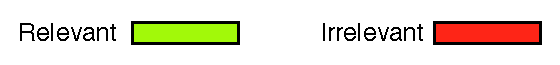
\includegraphics[width=4.5cm]{../img/legend} 
\par\end{centering}
\begin{centering}
\subfigure[Title query.]{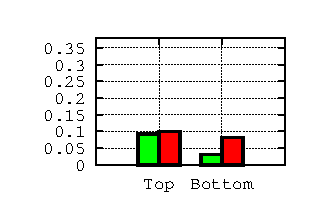
\includegraphics[width=3.5cm]{../Results-CIKM2014/jaccard-qTitle-CLEF-IP2010}}\subfigure[Abstract query.]{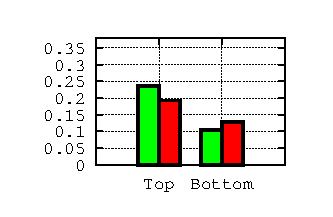
\includegraphics[width=3.5cm]{../Results-CIKM2014/jaccard-qAbstract-CLEF-IP2010}} 
\par\end{centering}

\begin{centering}
\subfigure[Claims query.]{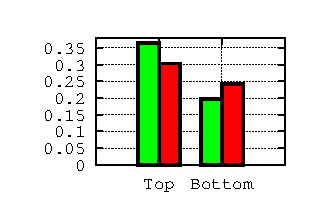
\includegraphics[width=3.5cm]{../Results-CIKM2014/jaccard-qClaims-CLEF-IP2010}}\subfigure[Description query.]{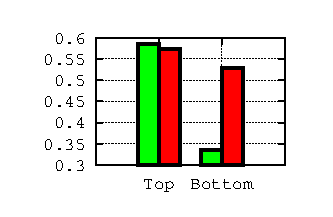
\includegraphics[width=3.5cm]{../Results-CIKM2014/jaccard-qDescription-CLEF-IP2010}}
\par\end{centering}
\end{figure}
\end{frame}


\begin{frame}
\frametitle{Term overlap between (ir)relevant documents with the results sets 
for different queries}

top 10 irrelevant documents ranked by BM25~\cite{Robertson1993}

Top 100 and bottom 100 queries (100 queries that perform the best, and 100 queries that perform the worst) CLEP-IP 2010 
% evaluated according to Mean Average Precision (MAP). 
There are 3 notable trends here: 
\begin{itemize}
\item[] 	(i) term overlap increases from title to description
since the query size grows accordingly; 
\item[]	(ii) the bottom 100 performing queries tend to have much smaller term overlap with the relevant documents than the top 100 queries; 
\item[]	(iii) the best overlap for any relevant
document set for any set of queries is less than one in four terms.
\end{itemize}
We investigate query formulation methods
\end{frame}



\begin{frame}
\frametitle{Query Reformulation}

Is the process of transforming an initial query $Q$ to another query $Q'$. 

\textbf{Query Reduction} (QR) \cite{Kumaran2009}: reduces the query such that superfluous information is removed,
\textbf{Query Expansion} (QE) \cite{Efthimiadis1996}: enhance the query with
additional terms likely to occur in relevant documents

Intensive study about query reformulation for patent
prior art search with partial patent applications

Contributions are the following: 
\begin{enumerate}
\item Novel contributions for query expansion and reduction that leverage
(a) patent structure and (b) term diversification techniques. 
\item A thorough comparative analysis of existing and novel methods for
query expansion and reduction in patent prior-art search on standardized
datasets of CLEF-IP. 
\end{enumerate}
\end{frame}



\begin{frame}
\frametitle{Query Reformulation for patents}

\begin{small}
\begin{itemize}
\item [Query type:] title, abstract, claims or the description section
What part of a partial application an inventor
should write to obtain the best search results?

\item [Relevance model:]  For initial retrieval of documents in the \emph{pseudo-relevant} feedback set (PRF) and subsequent re-retrieval, a probabilistic approach represented by the popular BM25~\cite{Robertson1993} and vector space model (VSM) approach, TF-IDF~\cite{Salton1975}. 
%there are various options for the relevance ranking model. a probabilistic approach represented by the popular BM25~\cite{Robertson1993} algorithm, as well as a vector space model (VSM) approach, TF-IDF~\cite{Salton1975}. 
Which relevance model works best for query reformulation
for patent prior art search? 

\item [Query expansion source:]  title, abstract,
claims, and description sections as different term sources
Are the title words of particularly high value as expansion terms? 
* Note that this only applies to query expansion methods. 

\item [ Term selection method:] Rocchio~\cite{Salton1971} and new term selection
methods that we propose in the next sections
%We consider different term selection methods for query reformulation. We evaluate the performance of term selection using Rocchio~\cite{Salton1971} and new term selection %which is intended to address the high-recall nature of patent prior art search. 
Which term selection method works best, and with which configuration, i.e. query type, retrieval model, and term source for query expansion methods? 
\end{itemize}
\end{small}

\end{frame}


\begin{frame}
\frametitle{Query Expansion Frameworks}

large term mismatch between queries an
relevant documents. This term mismatch may be alleviated by QE methods.

Rocchio derives a score for each potential query expansion term and in practice, the top-$k$ scoring terms (often for $k\ll200$) are used to expand the query and are
weighted according to their Rocchio score during the second stage
of retrieval. 
%The caveat of this approach is that given a limited budget of $k$ expansion terms, there is no inherent guarantee that these terms ``cover'' all documents in the pseudo-relevant set.
\end{frame}



\begin{frame}
\frametitle{Maximal Marginal Relevance Query Expansion}

Result set diversification algorithm \emph{Maximal Marginal Relevance} (MMR)~\cite{Carbonell1998}, usually used for \textbf{diverse document selection} (multi-document summarization)

\textbf{diverse term selection}
to address the deficiency of Rocchio
\end{frame}


\begin{frame}
\frametitle{Notation used in MMRQE}

\begin{equation}
%t_{k}^{*}=\argmax_{t_{k}\notin T_{k-1}^{*}}\hspace{-0.3mm}[\lambda\cos(Q,t_{k})-\hspace{-0.3mm}(1-\lambda)\max_{t_{j}\in T_{k-1}^{*}}\cos(t_{j},t_{k})]
\end{equation}

% We begin our formal description of MMRQE by first defining some necessary notation. MMRQE takes as input a pseudo-relevant feedback set of $n$ documents (PRF), which is obtained after a retrieval for the initial query. From the PRF set, we build a document-term matrix of $n$ documents and $m$ terms as shown in Figure~\ref{fig:notation}, which uses a TF-IDF weighting for each document vector (row $d_{i}$ for $1\leq i\leq n$). However, as we will see shortly, the view that will be important for us in this work is instead the term vector (column $t_{j}$ for $1\leq j\leq m$). To represent the query $Q$ column vector in Figure~\ref{fig:notation} having a numerical entry for every document $d_{i}$, we found that computing the BM25 or TF-IDF score between each document $d_{i}$ and the query provided the best performance (in our experiments, the score used is given by the indicated relevance model).

% Given a query representation $Q$, we aim to select an optimal subset of $k$ terms $T_{k}^{*}\subset D$ (where $|T_{k}^{*}|=k$ and $k\ll|m|$) relevant to $Q$ but inherently different from each other (i.e., diverse). This can be achieved by building $T_{k}^{*}$ in a greedy manner by choosing the next optimal term $t_{k}^{*}$ given the previous set of optimal term selections $T_{k-1}^{*}=\{t_{1}^{*},\ldots,t_{k-1}^{*}\}$ (assuming $T_{0}^{*}=\emptyset$) using the MMR diverse selection criterion:

%Here, the first cosine similarity term measures relevance between the query $Q$ and possible expansion term $t_{k}$ while the second term penalizes the possible expansion term according to it's cosine similarity with any currently selected term in $T_{k-1}^{*}$. The parameter $\lambda\in[0,1]$ trades off relevance and diversity and we found $\lambda=0.5$ to generally provide the best results in our experiments on the CLEF-IP training dataset collection.

\end{frame}



\begin{frame}
\frametitle{Query Reduction Frameworks }

While the title is usually composed by an average of six terms, the
other sections are longer, ranging from ten to thousands of terms.
Therefore, we investigate the impact of query reduction methods when
querying with long sections such as abstract, claims or description.

\end{frame}



\begin{frame}
\frametitle{Sample of terms removed from the abstract section}

\begin{figure}
\begin{center}
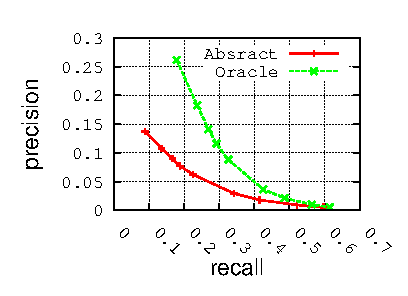
\includegraphics[width=4cm]{../analysis/precision-recall_ByField-CLEF-IP_2010}
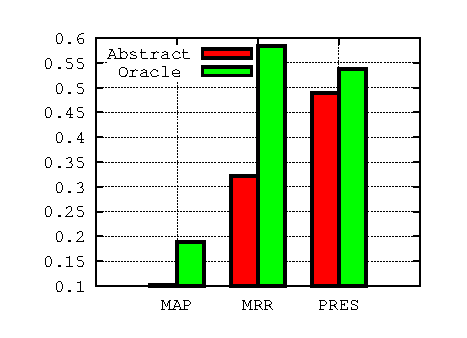
\includegraphics[width=4cm]{../analysis/MAP-MRR_ByField-CLEF-IP_2010}
\end{center}
\end{figure}

\end{frame}



\begin{frame}
\frametitle{The utility of query reduction for 1304 abstract queries of the CLEF-IP 2010 dataset}

\begin{tiny}
\begin{table}[h]
\begin{centering}
%\caption{Sample of terms removed from the abstract section of CLEP-IP2010 Topic PAC-1019. }
\par\end{centering}

\begin{centering}
{\footnotesize{}}
\par\end{centering}{\footnotesize \par}

\centering{}{\scriptsize{}}%
\begin{tabular}{|l|c|c|c|c|c|}
\hline 
\multicolumn{6}{|>{\raggedright}p{8cm}|}{\textbf{\scriptsize{}Topic:}{\scriptsize{} PAC-1019}}\tabularnewline
\hline 
\multicolumn{6}{|>{\raggedright}p{8cm}|}{\textbf{\scriptsize{}Abstract:}{\scriptsize{} A 5-aminolevulinic acid
salt which is useful in fields of microorganisms, fermentation, animals,
medicaments, plants and the like; a process for producing the same;
a medical composition comprising the same; and a plant activator composition
comprising the same.}}\tabularnewline
\hline 
\hline 
\textbf{\scriptsize{}Term removed} & \textbf{\scriptsize{}P@5} & \textbf{\scriptsize{}P@10} & \textbf{\scriptsize{}R@10} & \textbf{\scriptsize{}AP} & \textbf{\scriptsize{}PRES}\tabularnewline
\hline 
{\scriptsize{}composit...} & \textbf{\scriptsize{}0.600} & {\scriptsize{}0.300} & {\scriptsize{}0.428} & \textbf{\scriptsize{}0.360} & \textbf{\scriptsize{}0.829}\tabularnewline
\hline 
{\scriptsize{}activ...} & {\scriptsize{}0.400} & {\scriptsize{}0.300} & {\scriptsize{}0.428} & {\scriptsize{}0.277} & \textbf{\scriptsize{}0.809}\tabularnewline
\hline 
{\scriptsize{}anim...} & \textbf{\scriptsize{}0.600} & {\scriptsize{}0.300} & {\scriptsize{}0.428} & \textbf{\scriptsize{}0.345} & \textbf{\scriptsize{}0.798}\tabularnewline
\hline 
{\scriptsize{}produc...} & {\scriptsize{}0.400} & {\scriptsize{}0.300} & {\scriptsize{}0.428} & \textbf{\scriptsize{}0.286} & \textbf{\scriptsize{}0.797}\tabularnewline
\hline 
{\scriptsize{}ferment...} & {\scriptsize{}0.200} & {\scriptsize{}0.300} & {\scriptsize{}0.428} & \textbf{\scriptsize{}0.283} & \textbf{\scriptsize{}0.796}\tabularnewline
\hline 
{\scriptsize{}microorgan...} & \textbf{\scriptsize{}0.600} & {\scriptsize{}0.300} & {\scriptsize{}0.428} & \textbf{\scriptsize{}0.333} & \textbf{\scriptsize{}0.793}\tabularnewline
\hline 
{\scriptsize{}compris...} & {\scriptsize{}0.400} & {\scriptsize{}0.300} & {\scriptsize{}0.428} & {\scriptsize{}0.271} & \textbf{\scriptsize{}0.790}\tabularnewline
\hline 
{\scriptsize{}medica...} & {\scriptsize{}0.400} & {\scriptsize{}0.300} & {\scriptsize{}0.428} & \textbf{\scriptsize{}0.297} & \textbf{\scriptsize{}0.789}\tabularnewline
\hline 
{\scriptsize{}medic...} & {\scriptsize{}0.400} & {\scriptsize{}0.300} & {\scriptsize{}0.428} & \textbf{\scriptsize{}0.297} & \textbf{\scriptsize{}0.787}\tabularnewline
\hline 
{\scriptsize{}field...} & {\scriptsize{}0.400} & {\scriptsize{}0.300} & {\scriptsize{}0.428} & \textbf{\scriptsize{}0.282} & \textbf{\scriptsize{}0.782}\tabularnewline
\hline 
{\scriptsize{}plant...} & {\scriptsize{}0.200} & {\scriptsize{}0.200} & {\scriptsize{}0.285} & {\scriptsize{}0.114} & {\scriptsize{}0.774}\tabularnewline
\hline 
{\scriptsize{}process...} & {\scriptsize{}0.400} & {\scriptsize{}0.300} & {\scriptsize{}0.428} & {\scriptsize{}0.279} & {\scriptsize{}0.764}\tabularnewline
\hline 
{\scriptsize{}acid...} & {\scriptsize{}0.400} & {\scriptsize{}0.300} & {\scriptsize{}0.428} & {\scriptsize{}0.252} & {\scriptsize{}0.693}\tabularnewline
\hline 
{\scriptsize{}salt...} & {\scriptsize{}0.200} & {\scriptsize{}0.200} & {\scriptsize{}0.285} & {\scriptsize{}0.216} & {\scriptsize{}0.663}\tabularnewline
\hline 
{\scriptsize{}aminolevulin...} & {\scriptsize{}0.000} & {\scriptsize{}0.100} & {\scriptsize{}0.142} & {\scriptsize{}0.026} & {\scriptsize{}0.352}\tabularnewline
\hline 
\hline 
\textbf{\scriptsize{}Baseline} & {\scriptsize{}0.400} & {\scriptsize{}0.300} & {\scriptsize{}0.428} & {\scriptsize{}0.280} & {\scriptsize{}0.777}\tabularnewline
\hline 
\end{tabular}
\end{table}
\end{tiny}


\end{frame}



\begin{frame}
\frametitle{Experiments}

Setup


\end{frame}



\begin{frame}
\frametitle{Experiments results for QE}
\end{frame}



\begin{frame}
\frametitle{Discussion abut QE}
\end{frame}



\begin{frame}
\frametitle{Experiments results for QR}
\end{frame}



\begin{frame}
\frametitle{Discussion about QR}
\end{frame}



\begin{frame}
\frametitle{}
\end{frame}



\begin{frame}
\frametitle{}
\end{frame}



\begin{frame}
\frametitle{}
\end{frame}



\begin{frame}
\frametitle{}
\end{frame}


\begin{frame}
\frametitle{}
\end{frame}


\begin{frame}
\frametitle{}
\end{frame}


\begin{frame}
\frametitle{}
\end{frame}


\begin{frame}
\frametitle{}
\end{frame}


\begin{frame}
\frametitle{}
\end{frame}


\begin{frame}
\frametitle{}
\end{frame}


\begin{frame}
\frametitle{}
\end{frame}


\begin{frame}
\frametitle{}
\end{frame}


\begin{frame}
\frametitle{}
\end{frame}





\end{document}
